\begin{frame}[fragile]
  \frametitle{M\'odulos y paquetes}

  \framesubtitle{M\'odulos}

  Si se quisiera utilizar la funcionalidad definida en el m\'odulo anterior en nuestro programa se necesita importarlo.

  \begin{figure}
    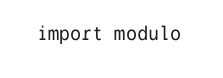
\includegraphics[width=0.6\textwidth]{Imagenes/Import.jpg}
    \caption{\label{fig:Ejemplo11}Sintaxis de import en Python.} 
  \end{figure}

  El import no solo hace que tengamos disponible todo lo definido dentro del m\'odulo, sino que tambi\'en ejecuta el c\'odigo dentro de \'el. 

\end{frame}
